\chapter{Introduction}\label{ch:introduction}

This report details a project done in Wireless Sensor Networks (WSN) with a mini-project called "To hop or to hop". The project follows the original idea of determining when to relay packets in a wireless network, but with a little twist to it - instead of placing the receiving node in a fixed position, we place it on an athlete running a marathon on a oval-formed running track in order to measure his heart rate every minute. This information is going to be transfered to a sink (base station) over a wireless connection with an added two relay stations in between that help ensure sufficient network coverage of the track. To design the track for our purpose, we will employ knowledge of fading, radio wave propagation and received input power (dbM) in a wireless node.

\noindent We will look to create an effective protocol that can determine when to communicate directly with the node based on the athlete and when it is best to use one of the relays. This protocol will take signal strength and energy consumption into consideration. For inter-node connectivity, we will design and implement the data-link layer stop-and-wait ARQ protocol on all nodes.

\noindent With reference to the mini-project presentation, we use telosb nodes all running TinyOS with a packet size of 128 bytes. The RF transceiver is a single-chip 2.4 GHz IEEE 802.15.4 compliant CC2420 with a data rate of 250 kbps.

\section{Scenario Introduction}\label{sc:scenarioIntroduction}
% Scenario introduction
A marathon runner is racing a track shaped as shown in figure 1, while equipped with sensor node A. The sensor node is broadcasting four packages per second tracking the runner’s pulse history. The level of details in the tracking package defines the number of marathons possible for the runner to run before a new battery is required. At one time the track was closed, resulting in the runner racing around the building of her workplace.

\begin{figure}[H]
	\centering
	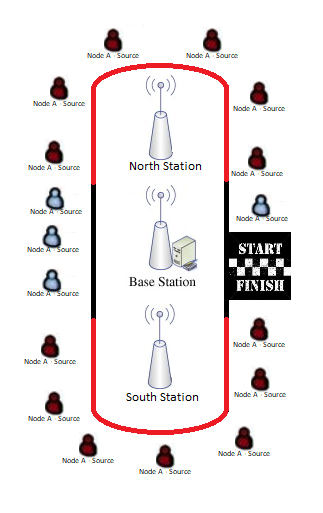
\includegraphics[width=\linewidth]{introduction/scenario/fig/scenarioIntroduction.png}
	\caption{A marathon runner "node A" is racing around a track, while transmitting pulse information to the base station. In the red northern territory, node A transmits to the north station which relays the message to the base station. Likewise, at the southern station.}
	\label{fig:scenarioIntroduction}
\end{figure}

\section{Protocol introduction “To hop or not to hop”}\label{sc:protocolIntroduction}
Node A will be broadcasting with a packet size of 128 Bytes. The base station will collect the data from node A when in range and save the data. The North station will, when in range and the base station is out of range, receive and relay the message to the base station. The same scenario will happen at the south station. Time Synchronization, Localization and Scalability will be considered regarding the protocol design. Each and combined scenarios will be evaluated in relation to signal strength relative to power consumption and data reliability. 
